\documentclass{beamer}

%\usetheme[secheader]{Boadilla}
\usetheme{Boadilla}
\usecolortheme{beetle}
\usepackage[latin1]{inputenc}
\usepackage{listings} % for code syntax highlighting
\usepackage{color}
\usepackage{caption}

%%%%%%%%%%%%%%%%%%%%%%%%%%%%%%%%%%%%%%%%%%%%%%%%%%%%%%%%%%%%%%%%%%%%%%%%%%%
%                                  Fonts                                  %
%%%%%%%%%%%%%%%%%%%%%%%%%%%%%%%%%%%%%%%%%%%%%%%%%%%%%%%%%%%%%%%%%%%%%%%%%%%


\usepackage{inconsolata} % for code
\usepackage{lmodern}
\renewcommand*\familydefault{\sfdefault} 
\usepackage[T1]{fontenc}

%%%%%%%%%%%%%%%%%%%%%%%%%%%%%%%%%%%%%%%%%%%%%%%%%%%%%%%%%%%%%%%%%%%%%%%%%%%
%                         Beamer Theme and colors                         %
%%%%%%%%%%%%%%%%%%%%%%%%%%%%%%%%%%%%%%%%%%%%%%%%%%%%%%%%%%%%%%%%%%%%%%%%%%%

 
\definecolor{gray}{HTML}{3A3A3A}
\definecolor{codebg}{HTML}{2C2C2C} % dark gray
\definecolor{codefg}{HTML}{D0D0D0} % light gray
\definecolor{themeblue}{HTML}{789FEF} % light blue
\definecolor{codecomment}{HTML}{808080} % gray
\definecolor{codestring}{HTML}{DFDF87} % for strings, light yellow
\definecolor{themedarkblue}{HTML}{1d2561}
\definecolor{themeyellow}{HTML}{DFDF67}

% tweak beamer theme
\setbeamercolor{framesubtitle}{fg=white}
\setbeamercolor{frametitle}{bg=codebg}
\setbeamercolor{title}{bg=codebg}
\setbeamercolor{palette primary}{bg=themedarkblue}
\setbeamercolor{author}{fg=white}
\setbeamercolor{date}{fg=white}
 
%%%%%%%%%%%%%%%%%%%%%%%%%%%%%%%%%%%%%%%%%%%%%%%%%%%%%%%%%%%%%%%%%%%%%%%%%%%
%                             Tweak Listings                              %
%%%%%%%%%%%%%%%%%%%%%%%%%%%%%%%%%%%%%%%%%%%%%%%%%%%%%%%%%%%%%%%%%%%%%%%%%%%

% caption stuff
\DeclareCaptionFormat{listing}{\parbox{\textwidth}{#1#2#3}}
\captionsetup[lstlisting]{format=listing}

\lstset{ %
  language=C++,                % the language of the code
  basicstyle=\small\ttfamily\color{codefg},           % the size of the fonts that are used for the code
  backgroundcolor=\color{codebg},      % choose the background color. You must add \usepackage{color}
  showspaces=false,               % show spaces adding particular underscores
  showstringspaces=false,         % underline spaces within strings
  showtabs=false,                 % show tabs within strings adding particular underscores
  %frame=single,                   % adds a frame around the code
  rulecolor=\color{black},        % if not set, the frame-color may be changed on line-breaks within not-black text (e.g. commens (green here))
  tabsize=2,                      % sets default tabsize to 2 spaces
  captionpos=t,                   % sets the caption-position to bottom
  breaklines=true,                % sets automatic line breaking
  breakatwhitespace=false,        % sets if automatic breaks should only happen at whitespace
  title=\lstname,                   % show the filename of files included with \lstinputlisting;
                                  % also try caption instead of title
  keywordstyle=\color{themeblue}\bfseries,
  stringstyle=\color{codestring},
  commentstyle=\color{codecomment},
  escapeinside={\%*}{*)},            % if you want to add LaTeX within your code
  morekeywords={*,...}               % if you want to add more keywords to the set
}
% ==========================================

%%%%%%%%%%%%%%%%%%%%%%%%%%%%%%%%%%%%%%%%%%%%%%%%%%%%%%%%%%%%%%%%%%%%%%%%%%%
%                     Custom Macros for Presentation                      %
%%%%%%%%%%%%%%%%%%%%%%%%%%%%%%%%%%%%%%%%%%%%%%%%%%%%%%%%%%%%%%%%%%%%%%%%%%%

% define a counter for rules
\newcounter{rulecount}
\newcommand{\declarerule}{\textbf{\color{themeblue}{Rule \therulecount:}} }

\newcommand{\declarelesson}{\textbf{\color{themeyellow}{Lesson:}} }

%%%%%%%%%%%%%%%%%%%%%%%%%%%%%%%%%%%%%%%%%%%%%%%%%%%%%%%%%%%%%%%%%%%%%%%%%%%
%                               Author info                               %
%%%%%%%%%%%%%%%%%%%%%%%%%%%%%%%%%%%%%%%%%%%%%%%%%%%%%%%%%%%%%%%%%%%%%%%%%%%


\title{Forgetting the C in C++}
\author{Alexander Kondratskiy}
\date{\today}
% \institute[2008]{ECON 101}

%%%%%%%%%%%%%%%%%%%%%%%%%%%%%%%%%%%%%%%%%%%%%%%%%%%%%%%%%%%%%%%%%%%%%%%%%%%
%                            Main Presentation                            %
%%%%%%%%%%%%%%%%%%%%%%%%%%%%%%%%%%%%%%%%%%%%%%%%%%%%%%%%%%%%%%%%%%%%%%%%%%%


\begin{document}

\frame{\titlepage}

\section{Introduction}
\frame{\sectionpage}

\frame {
    \frametitle{What is the talk about?}
    \begin{itemize}
        \item<2->Overview of C++, from a C programmer's perspective
        \item<2->Good C++ coding style
        \item<2->More than "C with classes"
        \item<2->Fixing bad habbits learnt from C.
    \end{itemize}
}

% Buzzwords
\frame {
    \frametitle{Motivation}
    \begin{itemize}
        \item<1->C++ has evolved
            % TODO: find word 
        \item<2->\alert{Safety}/Robustness
            \begin{itemize}
                \item Resource management (including memory)
                \item Type safety
                \item Compiler checks
            \end{itemize}
        \item<2->\alert{Readability}/Maintainability
            \begin{exampleblock}{}
                ``Programs must be written for people to read, and only incidentally for machines to execute.''
                \hspace*\fill{\small--- Abelson/Sussman, SICP}
            \end{exampleblock}
        \item<2->Programmer \alert{Productivity}
            \begin{itemize}
                \item STL
                \item Abstractions
            \end{itemize}
        \item<2->\alert{Efficiency} and speed
            \begin{itemize}
                \item More context for compiler
            \end{itemize}
        \item<3->Win-win
    \end{itemize}
}

% Guiding Principles
\begin{frame}
    \frametitle{Motivation}
    \framesubtitle{Guiding Principles}
    % TODO: move to STL?
    \begin{exampleblock}{}
        ``If I have seen further, it is by standing on the shoulders of giants''

        \hspace*\fill{\small--- Isaac Newton}
    \end{exampleblock}

    \begin{exampleblock}{}
        ``Make interfaces easy to use correctly and hard to use incorrectly''

        \hspace*\fill{\small--- Scott Meyers}
    \end{exampleblock}

\end{frame}

\begin{frame}
    \frametitle{Method}
    \begin{itemize}
        \item<1->Observe common C idiom
        \item<1->Discuss disadvantages
        \item<1->C++ alternative
        \item<1->Gains from the alternative
        \item<2->Learn new techniques/features along the way
    \end{itemize}
\end{frame}

\section{Prerequisites}
\frame{\sectionpage}

\begin{frame}
    \frametitle{History of C++}
    \begin{columns}[t]
        \column{7cm}
        \begin{itemize}
            \item<1->Started by Bjarne Stroustrup in 1979 as "C with Classes"
                \begin{itemize}
                    \item At Bell labs
                    \item "Down the hall" from Dennis Ritchie (creator of C)
                \end{itemize}
            \item<1->Renamed to C++ in 1983, commercially implemented in 1985
            \item<2->1990s: stream IO, STL, ISO Standard in 98
            \item<3->2000s: Boost, TR1 in 2007
            \item<4->2010s: C++11 in 2011
        \end{itemize}
        \column[T]{4cm}
        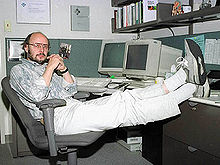
\includegraphics[width=4cm]{220px-BjarneStroustrup.jpg}
    \end{columns}
\end{frame}

% C Compilation
\begin{frame}
    \frametitle{C Compilation model}
    \framesubtitle{A single source file}
    \begin{columns}[t]
        \column{4cm}
        \begin{itemize}
            \item One source file at a time
            \item Preprocessor \emph{resolves all directives}
            \item Compiled to an object file
            \item Missing external function definitions
        \end{itemize}
        \column[T]{8cm}
        \includegraphics[height=9cm,angle=-90]{diagrams/c_compilation_model.pdf}
    \end{columns}
\end{frame}

% Linker
\begin{frame}
    \frametitle{C Compilation model}
    \framesubtitle{Linking}
    \begin{columns}[t]
        \column{4cm}
        \begin{itemize}
            \item Linker combines several translation units
            \item Resolves external dependencies
        \end{itemize}
        \column[T]{8cm}
        \includegraphics[height=9cm,angle=-90]{diagrams/c_compilation_model_linker.pdf}
    \end{columns}
\end{frame}

% Linker + Compiler large diagram
\begin{frame}
    \frametitle{C Compilation model}
    \framesubtitle{A typical project}
    \includegraphics[height=12cm,angle=-90]{diagrams/c_compilation_model_2.pdf}
\end{frame}

\begin{frame}
    \frametitle{\alert{C++} Compilation model}
    \begin{itemize}
        \item Same as C compilation model
        \item Template instantiation happens in the compiler
    \end{itemize}
\end{frame}

\section{Preprocessor}
\frame{\sectionpage}

\begin{frame}
    \frametitle{\declarerule Avoid the preprocessor}
    \begin{itemize}
        \item Macros are text substitution
        \item Macros not subject to scope rules
        \item Compiler does not see any preprocessor directives only final result of substitution
            \begin{itemize}
                \item No meaningful error checking!
            \end{itemize}
        \item Used naively can lead to subtle, hard to find bugs
    \end{itemize}
\end{frame}

\stepcounter{rulecount}
\begin{frame}[fragile]
    \frametitle{\declarerule Prefer \texttt{const} variables over \texttt{\#define}}
    \framesubtitle{Declaring constants}
\begin{lstlisting}
#define DAYSINWEEK 7
const unsigned int days_in_a_week = 7;
\end{lstlisting}
    \begin{itemize}
        \item Typesafe
            \begin{itemize}
                \item Unambiguous function overload usage
            \end{itemize}
        \item Debugging symbol exists
        \item Scoped
        \item Const variables can be any C++ type, not just numbers
            \begin{itemize}
                \item Can be pointed to
            \end{itemize}
    \end{itemize}
\end{frame}

% Beackerting problem
\stepcounter{rulecount}
\begin{frame}[fragile]
    \frametitle{\declarerule Avoid macro functions}
\begin{uncoverenv}<1->
\begin{lstlisting}[title=Given an innocent macro definition]
#define CIRCLE_AREA(R) 3.14 * R * R
\end{lstlisting}
\end{uncoverenv}

\begin{uncoverenv}<2->
\begin{lstlisting}[title=You write]
double total_area = 2 * CIRCLE_AREA( a + b );
\end{lstlisting}
\end{uncoverenv}

\begin{uncoverenv}<3->
\begin{lstlisting}[title=The compiler sees]
double total_area = 2 * 3.14 * a + b * a + b;
\end{lstlisting}
\begin{itemize}
    \item This code compiles with no errors,
        but is clearly not what is intended
\end{itemize}
\end{uncoverenv}

\end{frame}

% Fixing macro problem with brackets
\begin{frame}[fragile]
    \frametitle{\declarerule Avoid macro functions}
\begin{lstlisting}[title=\textbf{Macro Solution:} Wrap everything in brackets]
#define CIRCLE_AREA(R) (3.14 * (R) * (R))
\end{lstlisting}
\begin{itemize}
    \item<2->Macro functions do not work as functions
    \item<2->This solution is just a bandaid!
    \item<3->But wait... There's more!
\end{itemize}
\end{frame}

% Demonstrate problem with multiline macros
\begin{frame}[fragile]
    \frametitle{\declarerule Avoid macro functions}
    \framesubtitle{Multiline Macros}
    
\begin{uncoverenv}<1->
\begin{lstlisting}[title=A multiline macro that swaps the values of two variables]
#define SWAP(x, y) \
    tmp = x; \
    x = y; \
    y = tmp
\end{lstlisting}

\begin{lstlisting}[title=You write]
if (z == 0)
    SWAP( x, y);
\end{lstlisting}
\end{uncoverenv}

\begin{uncoverenv}<2->
\begin{lstlisting}[title=The compiler sees]
if (z == 0)
    tmp = x;
x = y;
y = tmp;
\end{lstlisting}
\end{uncoverenv}
\end{frame}

% Fix multiline with do while
\begin{frame}[fragile]
    \frametitle{\declarerule Avoid macro functions}
    \framesubtitle{Multiline Macros}
    
    \begin{lstlisting}[title=\textbf{Bandaid solution:} wrap in do-while]
#define SWAP(x, y) \
    do { \
        tmp = x; \
        x = y; \
        y = tmp; \
    } while (0)
\end{lstlisting}
\begin{itemize}
    \item Surely we can get by with bandaids!
\end{itemize}
\end{frame}

% Fix multiline with do while
\begin{frame}[fragile]
    \frametitle{\declarerule Avoid macro functions}
    \framesubtitle{Undefined Behaviour}
    
\begin{uncoverenv}<1->
\begin{lstlisting}[title=A simple abs macro]
#define ABS(x) (((x) < 0) ? -(x) : (x))
\end{lstlisting}

\begin{lstlisting}[title=You write]
m = ABS(++n); 
\end{lstlisting}
\end{uncoverenv}

\begin{uncoverenv}<2->
\begin{lstlisting}[title=The compiler sees]
m = (((++n) < 0) ? -(++n) : (++n))
/* undefined behaviour */
\end{lstlisting}
    \begin{itemize}
        \item Cannot modify object more than once in an expression.
        \item We've run out of bandaids!
    \end{itemize}
\end{uncoverenv}
\end{frame}

% Show solution to macro woes
\begin{frame}[fragile]
    \frametitle{\declarerule Avoid macro functions}
    \framesubtitle{Use inline functions}
\begin{lstlisting}[title=\textbf{Better solution:} inline functions]
inline double circle_area(double radius) {
    return 3.14 * radius * radius;
}
\end{lstlisting}

\begin{lstlisting}
inline void swap(int& x, int& y) {
    int temp = x;
    x = y;
    y = temp;
}
\end{lstlisting}

\begin{lstlisting}
inline double abs(double radius) {
    return (x < 0) ? -x : x);
}
\end{lstlisting}

\end{frame}

% Advantages of inline functions over macros
\begin{frame}[fragile]
    \frametitle{\declarerule Avoid macro functions}
    \framesubtitle{Use inline functions}
    \begin{itemize}
        \item<1->Use inline functions!
            \begin{itemize}
                \item Type safe
                \item Efficient- inlined by compiler
                \item Checked by compiler
                \item Scoped
                \item Can be used in C too
            \end{itemize}
        \item<2->Can we make them type-generic, like macros?
    \end{itemize}
\end{frame}

% Template inline functions
\begin{frame}[fragile]
    \frametitle{\declarerule Avoid macro functions}
    \framesubtitle{C++ to the rescue: templates!}
\begin{lstlisting}
template <typename T>
inline void swap(T& x, T& y) {
    T temp = x;
    x = y;
    y = temp;
}
\end{lstlisting}

\begin{lstlisting}
template <typename T>
inline T abs(T radius) {
    return (x < 0) ? -x : x);
}
\end{lstlisting}
\begin{itemize}
    \item All the advantages of functions
    \item Plus type-generic
\end{itemize}
\end{frame}

\begin{frame}
    \frametitle{\declarelesson Classes}
    
\end{frame}

\end{document}
